%%%%%%%%%%%%%%%%%%%%%%%%%%%%%%%%%%%%%%%%
% datoteka diploma-vzorec.tex
%
% vzorčna datoteka za pisanje diplomskega dela v formatu LaTeX
% na UL Fakulteti za računalništvo in informatiko
%
% vkup spravil Gašper Fijavž, december 2010
% 
%
%
% verzija 12. februar 2014 (besedilo teme, seznam kratic, popravki Gašper Fijavž)
% verzija 10. marec 2014 (redakcijski popravki Zoran Bosnić)
% verzija 11. marec 2014 (redakcijski popravki Gašper Fijavž)
% verzija 15. april 2014 (pdf/a 1b compliance, not really - just claiming, Damjan Cvetan, Gašper Fijavž)
% verzija 23. april 2014 (privzeto cc licenca)
% verzija 16. september 2014 (odmiki strain od roba)
% verzija 28. oktober 2014 (odstranil vpisno številko)
% verija 5. februar 2015 (Literatura v kazalu, online literatura)
% verzija 25. september 2015 (angl. naslov v izjavi o avtorstvu)
% verzija 26. februar 2016 (UL izjava o avtorstvu)
% verzija 16. april 2016 (odstranjena izjava o avtorstvu)
% verzija 5. junij 2016 (Franc Solina dodal vrstice, ki jih je označil s svojim imenom)


\documentclass[a4paper, 12pt]{book}
%\documentclass[a4paper, 12pt, draft]{book}  Nalogo preverite tudi z opcijo draft, ki vam bo pokazala, katere vrstice so predolge!



\usepackage[utf8x]{inputenc}   % omogoča uporabo slovenskih črk kodiranih v formatu UTF-8
\usepackage[slovene,english]{babel}    % naloži, med drugim, slovenske delilne vzorce
\usepackage[pdftex]{graphicx}  % omogoča vlaganje slik različnih formatov
\usepackage{fancyhdr}          % poskrbi, na primer, za glave strani
\usepackage{amssymb}           % dodatni simboli
\usepackage{amsmath}           % eqref, npr.
%\usepackage{hyperxmp}
\usepackage[hyphens]{url}  % dodal Solina
\usepackage{comment}       % dodal Solina

\usepackage[pdftex, colorlinks=true,
						citecolor=black, filecolor=black, 
						linkcolor=black, urlcolor=black,
						pagebackref=false, 
						pdfproducer={LaTeX}, pdfcreator={LaTeX}, hidelinks]{hyperref}

\usepackage{color}       % dodal Solina
\usepackage{soul}       % dodal Solina
\usepackage{algorithm}
\usepackage{algpseudocode}
\usepackage{lmodern}
\usepackage{amssymb}
\usepackage{listings}
\usepackage[font=small,labelfont=bf]{caption}
\usepackage{mathtools}
\DeclarePairedDelimiter{\ceil}{\lceil}{\rceil}
\usepackage{multirow}
\usepackage{amsmath}

%%%%%%%%%%%%%%%%%%%%%%%%%%%%%%%%%%%%%%%%
%	DIPLOMA INFO
%%%%%%%%%%%%%%%%%%%%%%%%%%%%%%%%%%%%%%%%
\newcommand{\ttitle}{Bayesovska optimizacija hiperparametrov v strojnem učenju}
\newcommand{\ttitleEn}{Bayesian optimization of hyperparameters in machine learning}
\newcommand{\tsubject}{\ttitle}
\newcommand{\tsubjectEn}{\ttitleEn}
\newcommand{\tauthor}{David Ocepek}
\newcommand{\tkeywords}{Bayesovka optimizacija, nastavljanje hiperparametrov, avtomatizirano strojno učenje}
\newcommand{\tkeywordsEn}{Bayesian optimization,  hyperparameter tunning, automated machine learning}


%%%%%%%%%%%%%%%%%%%%%%%%%%%%%%%%%%%%%%%%
%	HYPERREF SETUP
%%%%%%%%%%%%%%%%%%%%%%%%%%%%%%%%%%%%%%%%
\hypersetup{pdftitle={\ttitle}}
\hypersetup{pdfsubject=\ttitleEn}
\hypersetup{pdfauthor={\tauthor, do8572@fri.uni-lj.si}}
\hypersetup{pdfkeywords=\tkeywordsEn}


 


%%%%%%%%%%%%%%%%%%%%%%%%%%%%%%%%%%%%%%%%
% postavitev strani
%%%%%%%%%%%%%%%%%%%%%%%%%%%%%%%%%%%%%%%%  

\addtolength{\marginparwidth}{-20pt} % robovi za tisk
\addtolength{\oddsidemargin}{40pt}
\addtolength{\evensidemargin}{-40pt}

\renewcommand{\baselinestretch}{1.3} % ustrezen razmik med vrsticami
\setlength{\headheight}{15pt}        % potreben prostor na vrhu
\renewcommand{\chaptermark}[1]%
{\markboth{\MakeUppercase{\thechapter.\ #1}}{}} \renewcommand{\sectionmark}[1]%
{\markright{\MakeUppercase{\thesection.\ #1}}} \renewcommand{\headrulewidth}{0.5pt} \renewcommand{\footrulewidth}{0pt}
\fancyhf{}
\fancyhead[LE,RO]{\sl \thepage} 
%\fancyhead[LO]{\sl \rightmark} \fancyhead[RE]{\sl \leftmark}
\fancyhead[RE]{\sc \tauthor}              % dodal Solina
\fancyhead[LO]{\sc Diplomska naloga}     % dodal Solina


\newcommand{\BibTeX}{{\sc Bib}\TeX}

%%%%%%%%%%%%%%%%%%%%%%%%%%%%%%%%%%%%%%%%
% naslovi
%%%%%%%%%%%%%%%%%%%%%%%%%%%%%%%%%%%%%%%%  


\newcommand{\autfont}{\Large}
\newcommand{\titfont}{\LARGE\bf}
\newcommand{\clearemptydoublepage}{\newpage{\pagestyle{empty}\cleardoublepage}}
\setcounter{tocdepth}{1}	      % globina kazala

%%%%%%%%%%%%%%%%%%%%%%%%%%%%%%%%%%%%%%%%
% konstrukti
%%%%%%%%%%%%%%%%%%%%%%%%%%%%%%%%%%%%%%%%  
\newtheorem{izrek}{Izrek}[chapter]
\newtheorem{trditev}{Trditev}[izrek]
\newenvironment{dokaz}{\emph{Dokaz.}\ }{\hspace{\fill}{$\Box$}}

%%%%%%%%%%%%%%%%%%%%%%%%%%%%%%%%%%%%%%%%%%%%%%%%%%%%%%%%%%%%%%%%%%%%%%%%%%%%%%%
%% PDF-A
%%%%%%%%%%%%%%%%%%%%%%%%%%%%%%%%%%%%%%%%%%%%%%%%%%%%%%%%%%%%%%%%%%%%%%%%%%%%%%%


%%%%%%%%%%%%%%%%%%%%%%%%%%%%%%%%%%%%%%%% 
% define medatata
%%%%%%%%%%%%%%%%%%%%%%%%%%%%%%%%%%%%%%%% 
\def\Title{\ttitle}
\def\Author{\tauthor, matjaz.kralj@fri.uni-lj.si}
\def\Subject{\ttitleEn}
\def\Keywords{\tkeywordsEn}

%%%%%%%%%%%%%%%%%%%%%%%%%%%%%%%%%%%%%%%% 
% \convertDate converts D:20080419103507+02'00' to 2008-04-19T10:35:07+02:00
%%%%%%%%%%%%%%%%%%%%%%%%%%%%%%%%%%%%%%%% 
\def\convertDate{%
    \getYear
}

{\catcode`\D=12
 \gdef\getYear D:#1#2#3#4{\edef\xYear{#1#2#3#4}\getMonth}
}
\def\getMonth#1#2{\edef\xMonth{#1#2}\getDay}
\def\getDay#1#2{\edef\xDay{#1#2}\getHour}
\def\getHour#1#2{\edef\xHour{#1#2}\getMin}
\def\getMin#1#2{\edef\xMin{#1#2}\getSec}
\def\getSec#1#2{\edef\xSec{#1#2}\getTZh}
\def\getTZh +#1#2{\edef\xTZh{#1#2}\getTZm}
\def\getTZm '#1#2'{%
    \edef\xTZm{#1#2}%
    \edef\convDate{\xYear-\xMonth-\xDay T\xHour:\xMin:\xSec+\xTZh:\xTZm}%
}

\expandafter\convertDate\pdfcreationdate 

%%%%%%%%%%%%%%%%%%%%%%%%%%%%%%%%%%%%%%%%
% get pdftex version string
%%%%%%%%%%%%%%%%%%%%%%%%%%%%%%%%%%%%%%%% 
\newcount\countA
\countA=\pdftexversion
\advance \countA by -100
\def\pdftexVersionStr{pdfTeX-1.\the\countA.\pdftexrevision}


%%%%%%%%%%%%%%%%%%%%%%%%%%%%%%%%%%%%%%%%
% XMP data
%%%%%%%%%%%%%%%%%%%%%%%%%%%%%%%%%%%%%%%%  
\usepackage{xmpincl}
\includexmp{pdfa-1b}

%%%%%%%%%%%%%%%%%%%%%%%%%%%%%%%%%%%%%%%%
% pdfInfo
%%%%%%%%%%%%%%%%%%%%%%%%%%%%%%%%%%%%%%%%  
\pdfinfo{%
    /Title    (\ttitle)
    /Author   (\tauthor, damjan@cvetan.si)
    /Subject  (\ttitleEn)
    /Keywords (\tkeywordsEn)
    /ModDate  (\pdfcreationdate)
    /Trapped  /False
}


%%%%%%%%%%%%%%%%%%%%%%%%%%%%%%%%%%%%%%%%%%%%%%%%%%%%%%%%%%%%%%%%%%%%%%%%%%%%%%%
%%%%%%%%%%%%%%%%%%%%%%%%%%%%%%%%%%%%%%%%%%%%%%%%%%%%%%%%%%%%%%%%%%%%%%%%%%%%%%%

\begin{document}
\selectlanguage{slovene}
\frontmatter
\setcounter{page}{1} %
\renewcommand{\thepage}{}       % preprecimo težave s številkami strani v kazalu
\newcommand{\sn}[1]{"`#1"'}                    % dodal Solina (slovenski narekovaji)

%%%%%%%%%%%%%%%%%%%%%%%%%%%%%%%%%%%%%%%%
%naslovnica
 \thispagestyle{empty}%
   \begin{center}
    {\large\sc Univerza v Ljubljani\\%
      Fakulteta za računalništvo in informatiko}%
    \vskip 10em%
    {\autfont \tauthor\par}%
    {\titfont \ttitle \par}%
    {\vskip 3em \textsc{DIPLOMSKO DELO\\[5mm]         % dodal Solina za ostale študijske programe
%    VISOKOŠOLSKI STROKOVNI ŠTUDIJSKI PROGRAM\\ PRVE STOPNJE\\ RAČUNALNIŠTVO IN INFORMATIKA}\par}%
    UNIVERZITETNI  ŠTUDIJSKI PROGRAM\\ PRVE STOPNJE\\ RAČUNALNIŠTVO IN INFORMATIKA}\par}%
%    INTERDISCIPLINARNI UNIVERZITETNI\\ ŠTUDIJSKI PROGRAM PRVE STOPNJE\\ RAČUNALNIŠTVO IN MATEMATIKA}\par}%
%    INTERDISCIPLINARNI UNIVERZITETNI\\ ŠTUDIJSKI PROGRAM PRVE STOPNJE\\ UPRAVNA INFORMATIKA}\par}%
%    INTERDISCIPLINARNI UNIVERZITETNI\\ ŠTUDIJSKI PROGRAM PRVE STOPNJE\\ MULTIMEDIJA}\par}%
    \vfill\null%
    {\large \textsc{Mentor}:  izr. prof. dr. Matjaž Kukar\par}%
    {\vskip 2em \large Ljubljana, 2020 \par}%
\end{center}
% prazna stran
%\clearemptydoublepage      % dodal Solina (izjava o licencah itd. se izpiše na hrbtni strani naslovnice)

%%%%%%%%%%%%%%%%%%%%%%%%%%%%%%%%%%%%%%%%
%copyright stran
\thispagestyle{empty}
\vspace*{8cm}

\noindent
{\sc Copyright}. 
Rezultati diplomske naloge so intelektualna lastnina avtorja in Fakultete za računalništvo in informatiko Univerze v Ljubljani.
Za objavo in koriščenje rezultatov diplomske naloge je potrebno pisno privoljenje avtorja, Fakultete za računalništvo in informatiko ter mentorja.

\begin{center}
\mbox{}\vfill
\emph{Besedilo je oblikovano z urejevalnikom besedil \LaTeX.}
\end{center}
% prazna stran
\clearemptydoublepage

%%%%%%%%%%%%%%%%%%%%%%%%%%%%%%%%%%%%%%%%
% stran 3 med uvodnimi listi
\thispagestyle{empty}
\vspace*{4cm}

\noindent
Fakulteta za računalništvo in informatiko izdaja naslednjo nalogo: \\
Bayesovska optimizacija hiperparametrov v strojnem učenju
\medskip
\begin{tabbing}
\hspace{32mm}\= \hspace{6cm} \= \kill




Tematika naloge:
\end{tabbing}
Osrednji cilj diplomske naloge je predstaviti in pregledati orodja za optimizacijo hiperparametrov s poudarkom na metodi Bayesovske optimizacije.
Opisati razloge za njeno uporabo, jo razdeliti na osnovne sestavne dele in le-te predstaviti.
Na koncu pa preizskusiti metodo na nekaj praktičnih primerih ter predstaviti in interpretirati dobljene rezultate.  
\vspace{15mm}






\vspace{2cm}

% prazna stran
\clearemptydoublepage

% prazna stran
\clearemptydoublepage

%%%%%%%%%%%%%%%%%%%%%%%%%%%%%%%%%%%%%%%%
% posvetilo, če sama zahvala ne zadošča :-)
\thispagestyle{empty}\mbox{}{\vskip0.20\textheight}\mbox{}\hfill\begin{minipage}{0.55\textwidth}%
\normalfont\end{minipage}

%%%%%%%%%%%%%%%%%%%%%%%%%%%%%%%%%%%%%%%%
% kazalo
\pagestyle{empty}
\def\thepage{}% preprecimo tezave s stevilkami strani v kazalu
\tableofcontents{}


% prazna stran
\clearemptydoublepage

%%%%%%%%%%%%%%%%%%%%%%%%%%%%%%%%%%%%%%%%
% seznam kratic

\chapter*{Seznam uporabljenih kratic}  % spremenil Solina, da predolge vrstice ne gredo preko desnega roba

\noindent\begin{tabular}{p{0.1\textwidth}|p{.4\textwidth}|p{.4\textwidth}}    % po potrebi razširi prvo kolono tabele na račun drugih dveh!
  {\bf kratica} & {\bf angleško}                             & {\bf slovensko} \\ \hline
  {\bf BO} & bayesian optimization & BO \\
  {\bf RS} & random search & naključno iskanje \\
  {\bf EI} & expected improvement & pričakovana izboljšava \\
  {\bf PI} & probability of improvement & verjetnost izboljšave \\
  {\bf LCB} & lower confidence bounds & spodnja meja zaupanja \\
  {\bf ES} & entropy search & entropijsko iskanje \\
  {\bf PES} & predictive entropy search & napovedno entropijsko iskanje \\
%  {\bf KG} & knowladge gradient & informirani gradient \\
  {\bf GP} & gaussian process & gausov proces \\
  {\bf CNN} & convolutional neural network & konvolucijska nevronska mreža \\
  {\bf CA} & classification accuracy & klasifikacijska točnost \\
  {\bf AUC} & area under the curve & površina pod krivuljo \\  
  {\bf TS} & thompson vzorčenje & thomson sampling \\
  {\bf ML} & machine learning  & strojno učenje \\
  {\bf autoML} & automated machine learning & avtomatizirano strojno učenje \\
  {\bf SVC} & support vector classifier & klasifikator podpornih vektorjev \\
  {\bf GS} & grid search & iskanje v mreži \\
%  \dots & \dots & \dots \\
\end{tabular}


% prazna stran
\clearemptydoublepage

%%%%%%%%%%%%%%%%%%%%%%%%%%%%%%%%%%%%%%%%
% povzetek
\addcontentsline{toc}{chapter}{Povzetek}
\chapter*{Povzetek}

\noindent\textbf{Naslov:} \ttitle
\bigskip

\noindent\textbf{Avtor:} \tauthor
\bigskip

%\noindent\textbf{Povzetek:} 
\noindent 
Opišemo vlogo metode BO na področju ML.
Spošno opišemo metodo BO, njene prednosti in slabosti.
BO razčlenimo po glavnih komponentah na verjetnostni model in odločilno funkcijo.
Vsako od glavnih komponent predstavimo.
Pri verjetnostnih modelih predstavimo GP ter analiziramo njene latnosti.
Pri odločilnih funkcijah predstavimo 3 uporabljene funkcije: EI, PI in LCB ter nekaj novejših funkcij.
Predstavimo izvedene experimente na različnih datasetih in modelih (CNN, SVM, GradientBoosting, RandomForests).
Pri experimentih analiziramo hitrost konvergence po iteracijah ter doseženo stopnjo optimizacije hiperparametrov.
Rezultate BO primerjamo z metodama RS in GS, pogosto uporabljanima metodama za optimizacijo hiperparametrov. 
BO v vseh experimentih in metrikah doseže enakovredne ali boljše rezultate od RS in GS.

\bigskip

\noindent\textbf{Ključne besede:} \tkeywords.
% prazna stran
\clearemptydoublepage

%%%%%%%%%%%%%%%%%%%%%%%%%%%%%%%%%%%%%%%%
% abstract
\selectlanguage{english}
\addcontentsline{toc}{chapter}{Abstract}
\chapter*{Abstract}

\noindent\textbf{Title:} \ttitleEn
\bigskip

\noindent\textbf{Author:} \tauthor
\bigskip

%\noindent\textbf{Abstract:} 
\noindent We describe the role of the BO method in ML.
We give a basic description and analyze BO its pros and cons.
We split BO into its main compenents: the probability model and acquisition function.
We introduce the probability model of GP and analyze its properties.
We introduce 3 used acquisition functions: EI, PI, LCB and some newer functions.
We perform experiments on different datasets and models (CNN, SVM, GradientBoosting, RandomForests).
For each experiment we analyze the speed of convergence and optimization results.
We compare the results of BO to RS and GS, two commonly used methods for hyperparameter optimization.
In all experiments and metrics BO performs equal or better than RS and GS.
\bigskip

\noindent\textbf{Keywords:} \tkeywordsEn.
\selectlanguage{slovene}
% prazna stran
\clearemptydoublepage

%%%%%%%%%%%%%%%%%%%%%%%%%%%%%%%%%%%%%%%%
\mainmatter
\setcounter{page}{1}
\pagestyle{fancy}

\chapter{Uvod}
\par ML je bilo v zadnjih desetletjih priča številnim napredkom.
Te napredki so s sabo prinesli bolj natančne in hkrati bolj kompleksne modele.
Te modeli imajo množico nastavljivih parametrov, imenovanih hiperparametri.
Optimalne vrednosti teh hiperparametrov se razlikujejo od problema do problema, posledično je problem ročnega nastavljanja hiperparametrov časovno zahteven problem, ki zahteva veliko strokovnega znanja.
\par Zgodnje metode, ki so se soočale s tem problemom so bile tako imenovane ``model-free'' metode, ki niso uporabljale predhodno pridobljenega znanja.
 Primera teh metod sta GS ali GridSearch, ki iz diskretnega prostora kombinacij množic parametrov izbere kombinacijo, pri kateri model doseže maksimum glede na metrike uspešnosti.
Metoda ima polinomično časovno zahtevnost $\mathcal{O}(n^c)$, glede na število dimenzij $n$ in moč množice $c$. 
Boljša je metoda RS, ki naključno izbira točke v omejenem prostoru ter tako omogoča večjo pokritost posameznih dimenzij.
Metode RS in GS se uporabljata samo za podajanje kontexta za analizo in ovrednotenje rezultatov.
\par Razlog za to je velika  časovna zahtevnost potrebna za učenje samotnih modelov, kar pomeni da je število točk, ki jih lahko te funkcije ovrednotijo in preizkusijo pogosto omejeno na nekaj deset  ali stotero.
Zato se pogosteje uporabljajo bolj efektivne metode na podlagi modelov, ki pri izbiri točk za evaluacijo uporabljajo predhodno pridobljeno znanjo iz predhodno evaluiranih točk.
State of the art na tem področju je metoda BO, ki po vsaki evaluaciji točke posodablja model hiperravnine in na podlagi tega izbere naslednjo točko. 
Metoda hitreje konvergira kot zgoraj navedene metode in doseže boljše optimume kot RS in GS. 
V zadnjih par letih je BO podrla veliko benchmarkov, saj se je izkazalo, da razen tega, da strojno nastavljanje odstrani potrebo ročnem nastavljanju hiperparametrov ima še druge prednosti kot sta pridobivanje boljših rezultatov in boljša reproduktivnost raziskav in rezultatov.
\par Delo je sestavljeno iz n poglavij.
 V 2. poglavju predstavimo BO, zapišemo in obrazložimo osnovni algoritem BO.
 V 3. poglavju predstavimo sestavne dele BO optimizacije, in sicer model hiperravnine hiperparametrov in odločilno funkcijo, ki izbira naslednjo točko za evaluacijo.
 V 4. poglavju predstavimo predstavimo posamične eksperimente, modele in podatke, ki jih uporabljamo za posamezne eksperiment ter opišemo razlog in namen za izvedbo eksperimenta.
 V 5. poglavju predstavimo in analiziramo pridobljene rešitve ter ovrednotimo ali so bili eksperimenti uspešni.
 V zadnjem poglavju je predstavljen zaključek in sklep dela. 


\chapter{Bayesovska optimizacija}

\section{Osnovni pregled}

\par V tem poglavju na grobo predstavimo Bayesovsko optimizacijo.
Opišemo temeljne korake algoritma in obrazložimo kako se v algoritmu uporablja bayesovska statistika.
Predstavimo prednosti in slabosti grobega algoritma in morebitne izboljšave.
Na koncu pa podamo praktične primere uporabe.
\par Bayesovska optimizacija je iterativen algoritem za iskanje globalnega optimuma poljubne funkcije: 
\begin{equation}
	x^* = \operatornamewithlimits{argmin}_{x \epsilon X} f(x)
\end{equation}
Prednost Bayesovke optimizacija pred RS ali GS je, da je zelo podatkovno učinkovita, saj je bolj fokusirana na izboljšavo funkcije kot na samo preiskovanje prostora, kar je v praktičnih primerih zelo pomembno.
Razlog za to je, da je optimizirana funkcija sestavljena iz učenja in evaluiranja modela, zato lahko ena evaluacija tudi enostavnejšega modela traja več GPU ur.
V pogostih primerih uporabe cloud computinga pa so potrate tudi denarne in ne samo časovne.
\par Algoritem je sestavljen je iz dveh ključnih delov: 
verjetnostnega modela, ki na podlagi že znanih točk modelira verjetnostno hiperravnino, ki je sestavljena iz povprečja in standardnega odklona in
 odločilne funkcije, ki na podlagi verjetnostnega modela izbere naslednjo točko za evaluacijo. 
Apriorni verjetnostni model je v vsaki iteraciji posodobljen s podatki pridobljenimi v prejšnji iteraciji z uporabo bayesovske statistike.
Na podlagi pridobljenega posteriornega verjetnostnega modela potem odločilna funkcija izbere naslednjo točko.
Spodaj je podan osnovni algoritem za BO:

\begin{algorithm}[H]
	\caption{Bayesian optimization}\label{basic:bayesianOpt}
  	\begin{algorithmic}[1]
  		 \State \texttt{Inicializiraj X s naključnimi točkami in evaluiraj $y= f(X)$, natstavi $D_0 = (X, y)$.}
		\For{\texttt{ n = 1,2,...}}
			\State \texttt{posodobi statističen model}
			\State \texttt{$x_{n+1} = \operatornamewithlimits{argmax}_{x} \alpha(x; D_n)$}	\Comment \texttt{izberi $x_{n+1}$ v optimumu odločilne funkcije $\alpha$}
			\State \texttt{$y_{n+1} = f(x_{n+1})$}	\Comment \texttt{izračunaj vrednost funkcije v izbrani točki $x_{n+1}$}
			\State \texttt{$D_{n+1}=\{D_{n}, (x_{n+1}, y_{n+1})\}$} \Comment \texttt{posodobi tabelo znanih vrednosti podmnožice točk $X$}
		\EndFor
 	\end{algorithmic}
\end{algorithm}

Da bi bila Bayesovska optimizacija res uporabna pa mora veljati, da sta evaluacija verjetnostnega modela in odločilne funkcije v primerjavi s samo funkcijo $f$ vsaj par stopenj magnitude cenejša.
Na žalost pa je v praksi večina verjetnostnih modelov in odločilnih funkcij komputacijsko nerešljivih.
V praksi so uporabljani sestavni deli analitično rešljivi. 
\par Kot je bilo že zgoraj omenjeno je Bayesovska optimizacija bayesovska, zato ker uporablja bayesov teorem za posodabljanje verjetnosti v verjetnostnem modelu.

\begin{equation}
	P(A|B) = \frac{P(B|A)P(A)}{P(B)}
\end{equation}

Verjetnost $P(B)$ je v pogosto računsko nerešljiva na srečo ima samo vlogo normalizacije, zato ga pri računanju ne potrebujemo upoštevati in lahko predstavimo posteriorno verjetnost kot v odvisnosti od $P(B)$.

\begin{equation}
	P(A|B) = P(B|A)P(A)
\end{equation}

To lahko naredimo, zato ker nas točna verjetnost ne zanima, zanima nas samo optimizacija te verjetnosti. 
V našem primeru je $A = f$ in $B = D,x$.
Torej enačba izgleda takole:

\begin{equation}
	P(f|D,x) = P(D,x|f)P(D,x)
\end{equation}

Posteriorna verjetnost $P(f|D,x)$ predstavlja posodobljeno verjetnostni model funkcije $f$ za vsako točko $x$ glede na množico že znanih točk $D$, medtem ko apriorna verjetnost $P(D,x|f)$ verjetnost, je verjetnost obzervacije verjetnosti $f$ v točki $x$.
Apriorna verjetnost podaja verjetnostni model.
\par Za konec bi dodali še eno prednost bayesovske optimizacije in sicer njeno modularnost.
 Zaradi praktičnih razlogov je sicer izbira verjetnostnega modela in odločilnih funkcij omejena, vendar kljub temu obstajata vsaj dva v praksi uporabljana za verjetnostna modela ter veliko odločilnih funkcij, kar omogoča kombiniranje le-teh in izbiro najbolj primerne kombinacije za obravnavan problem.
 Za verjetnostni model se uporabljajo Gausovi procesi, ki so podobni multivariantni gausovi distribuciji in random forest.
 Izbira odločilnih funkcij je velika zato smo se v našem primeru omejili na pozneje opisane funkcije EI, PI in LCB.
\par Pogosto pa je kljub relativno hitri naravi teh komponent Bayesovska optimizacija še vedno prepočasna ali pa obstaja želja po več evaluacijah, zato obstajajo metode, ki pohitrijo algoritem za majhne izgube v natančnosti. 
Najenostavnejša in tudi najbolj pogosto časovna optimizacija je poganjati optimizirano funkcijo na podmnožici dataseta, treniranje algoritma na manjšem številu iteracij, na zmanjšani množici zančilk ter na eni ali nekaj prerezov pri prečni validaciji.

\section{Knjižnice}

\par Na območju bayesovske optimizacije obstaja mnogo knjižnic, v katerih je implementirana bayesovska optimizacija.
Primeri takih knjižnic so BayesianOptimization, GPyOpt, Spearmint, GPflowOpt, scikit-optimize, sklearn GPR in GPClassifier, hyperotp, optuna, HpBandSter, Botorch in verjetno še druge.

\chapter{Verjetnostni modeli}

\par V tem poglavju razložimo razliko med parametričnimi in neparametričnimi modeli, potem natančneje raziščemo najpogosteje uporabljan verjetnostni model GP, predstavimo razloge za njegovo uporabo, opišemo in razložimo njegovo teoretično podlago in podamo primere za lažje razumevanje.
\par Parametrični modeli $p(f|X,\theta)$ so modeli, ki imajo fiksno število parametrov.
Pogosto se uporabljajo pri strojnem učenju za razlago in modeliranje podatkov, pogosto pa uporabimo regresijo, da dobimo tak $\theta$, ki optimizira $p(f|X,\theta)$.
Glede na to da so dataseti čedalje večji in čedalje bolj kompleksni so potrebnimi modeli, ki imajo čedalje več parametrov.
Posledično so se začeli uporabljati neparametrični modeli.
Ime neparametrični je zavajajoče in ne pomeni, da modeli nimajo parametrov, ampak da jih imajo poljubno mnogo.
Eden s takih modelov so Gausovi procesi.
Grobo si lahko predstavljamo GP kot multivariantno funkcijo $f(x) = [\mu(x), \delta(x)]$, ki vsaki točki v prostoru hiperparametrov določi povprečje $\mu(x)$ in standardni odklon $\delta(x)$.

\begin{figure}[H]
\centerline{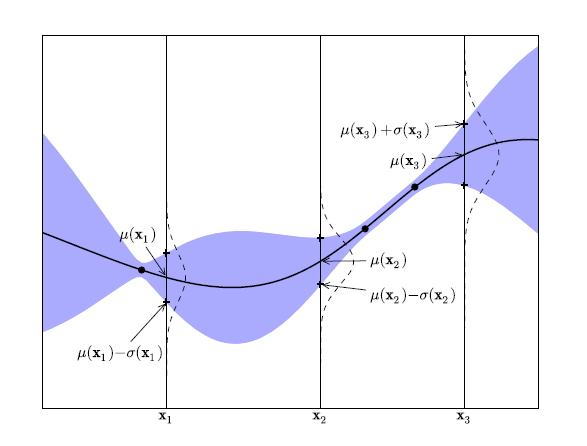
\includegraphics[height=0.5\textwidth]{images/gausian_simple_example}}
\caption{Enostaven 1D Gausov proces s tremi evaluiranimi točkami.
Črna črta predstavlja predpostavljano povprečje optimizirane funkcije glede na podatke in osenčeno območje okoli predstavlje povprečje plus ali minus standardna deviacija.
Prekrivajoče Gausove krivulje predstavljajo GP povprečje in standardno deviacijo v točkah $x_{1:3}$}
\label{1D Gausov proces}
\end{figure}

Za bolj natančno razumevanje pa je potrebno razumevanje multivariantne gausove distribucije, saj je prehod iz te na gausove procese zelo preprost.
\par Najprej predstavimo enostavno univariantno gausovo distribucijo $X \sim N(\mu, \sigma)$, ki se glasi

\begin{equation}
	p(x) = \frac{1}{\sqrt{2\pi\sigma^2}}e^{-\frac{1}{2\sigma^2}{(x-\mu)}^2}
\end{equation}

Enačba za multivariantno distribucijo $k$-dimenzionalno $X \sim N(\mu, \Sigma)$ je slednja

\begin{equation}
	p(x) = \frac{1}{\sqrt{2\pi\delta^k|\Sigma|}}e^{-\frac{1}{2}{(x-\mu)}^T\Sigma{(x-\mu)}}
\end{equation}

kjer je $\mu$ k-dimenzionalen vektor povprečnih vrednosti glede na vsako dimenzijo

\begin{equation}
	\mu = E[X] = (E[X_1],E[X_2],E[X_3],...,E[X_4])
\end{equation}

 in $\Sigma$ kovariančna matrika, kjer je $\Sigma (n,m)$ enako kovarianci med n-to in m-to gausovo ditribucijo.
 
 \begin{equation}
	\Sigma_{i,j} = E[(X_i - \mu_i)(X_j - \mu_j)] = Cov[X_i, X_j]
\end{equation}
 
Podobnost je pogosto v primeru Bayesovske optimizacije podana s posebno funcijo jedra $K$.
\par Medtem ko je multivariantna gausova distribucija porazdelitev nad vektorji je gausov proces porazdelitev nad funkcijami.

 \begin{equation}
	f(x) \sim GP(m(x), k(x, x^{'}))
\end{equation}

kjer je katerokoli končna podmnožica $X = {x_1, x_2..., x_n}$ v domeni $x$, porazdeljena multivariantno gausovo distribucijo:

\begin{equation}
	f(X) \sim N(m(X), k(X, X))
\end{equation}

Edina razlika med Gausovim procesom in distribucijo je, da gausov proces ni omejen končno število distribucij.

\section{Jedra}

Za gausove procese potrebujemo funkcijo $m(x)$ in kovariančno funkcijo podobnosti točk $k(x_i, x_j)$.
Funkcijo $m(x)$ se pogosto nastavi na $0$, saj so podatki normalizirani in kljub normalizaciji GP neizgubi na moči izražanja.
Za funkcijo $k(x_i, x_j)$ pa mora veljati, da točkam, ki pri evaluaciji so si blizu vrne visoko vrednost medtem ko bolj odaljenim točkam vrne različne vrednosti.
Pogosto se uporablja funkcija RBF ali radial basis function, ki ima naslednjo obliko:

\begin{equation}
	k(x_i, x_j) = e^{(-\frac{||x_i-x_j||^2}{2\delta^2})}
\end{equation}

$\delta$ je prost parameter in omogoča spreminjanje skale vhodov v funkcijo $k$.
V primeru, da je $\delta$ vektor je možno za vsak hiperparameter nastaviti skalo posebej.
To je potrebno in uporabno, saj imajo hiperparametri različna definicijska območja, ki jih je potrebno normalizirati za pravilno Gausovih procesov. 
Dodatna prednost tega jedra je, da je stacionarno, kar pomeni, da je ni odvisno od samih vrednosti $x_i$ in $x_j$ in je odvisno le od velikosti razdalje med njima.


\begin{figure}[H]
\centerline{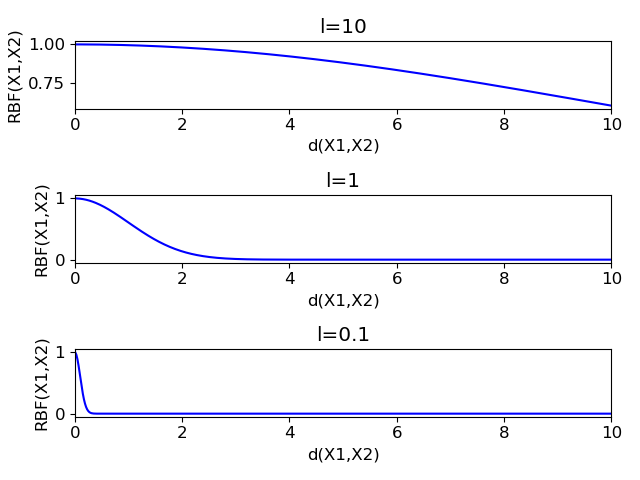
\includegraphics[height=0.6\textwidth]{images/RBF}}
\caption{Slika prikazuje RBF jedro s parametrom $l=10$, $l=1$ in $l=0.1$. 
Iz slike je razvidno, kako s večanjem parametra $l$ se večja predpostavljana razdalja na katerih so si točke še podobne podobnost točk, ki so si med sabo bolj oddaljene.
Funkcija je omejena samo na pozitivne vrednosti, saj je parameter $d$ vedno večji od 0.}
\label{RBF jedro}
\end{figure}

\par Posplošitev RBF jedra je družina pogosto uporabljanih stacionarnih jeder Matern, ki imajo slednjo obliko:

\begin{equation}
	C_v(d) = \sigma^2\frac{2^{1-\nu}}{\Gamma(\nu)}{(\sqrt{2\nu}\frac{d}{\rho})}^\nu K_\nu (\sqrt{2\nu}\frac{d}{\rho})
\end{equation}

kjer je $\Gamma$ gamma funkcija, $K_v$ je modificirana Bessel funkcija.
$\rho$ in $\nu$ sta prosta parametra funkcije.

Velja da lahko Gausov proces, ki uporablja Metern jedro $C_v$ odvajamo $\ceil{v} - 1$ krat.
V primeru, da je $x = 1$ je Matern jedro ekvivalentno exponentnemu jedru, medtem ko v $\lim_{v \to \infty}$ je jedro ekvivalentno jedru RBF.
V praksi se uporabljajo jedra oblike $v = p + 1/2$, kjer je $p$ pozitivno celo število.
Za to podmnožico Matern jeder je značilno, da imajo poenostavljeno analitično obliko.
Kot primer podamo najpogosteje uporabljano jedro Matern5/2.

\begin{equation}
	K_{5/2} = \sigma^2 (1 + \frac{\sqrt{5}d}{l} + \frac{5d^2}{3l^2})e^{-\frac{\sqrt{5}d}{l}}
\end{equation}

Matern5/2 je uporabljana v knnjižnici, ki je bila uporabljena za to diplomsko.
Spodaj je prikazan graf funkcije Matern5/2: 

\begin{figure}[H]
\centerline{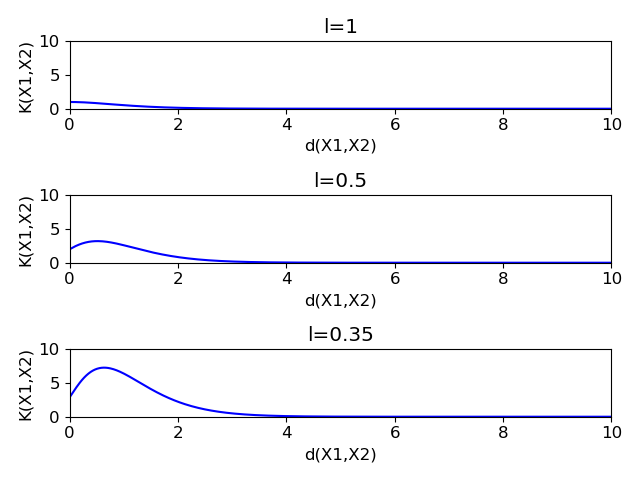
\includegraphics[height=0.6\textwidth]{images/matern}}
\caption{Slika prikazuje RBF jedro s parametrom $l=1$, $l=0.5$ in $l=0.35$. 
Iz slike je razvidno, da se s večanjem parametra $l$ večja predpostavljana razdalja  počasneje kot pri RBF ter da predpostavljana točka s največjo podobnostjo ni točka na razdalji nič, vendar malce oddaljena.
Funkcija je omejena samo na pozitivne vrednosti, saj je parameter $d$ vedno večji od 0.}
\label{Matern5/2 jedro}
\end{figure}

\section{Napovedovanje vrednosti GP}

Zdaj ko imamo jedro predstavimo enačbo verjetnostni funkcije $p(f|X)$:

\begin{equation}
	p(f,X) = N(f|\mu, K)
\end{equation}

V zgornji enački je $f = {[f(x_1), ..., f(x_N)]}^T$, $\mu = {[m(x_1), ..., m(x_N)]}^T$ in $K_{ij} = \kappa(x_i,x_j)$.
Pogosto uporabimo $m(x)=0$, saj je GP dovolj fleksibilen model, da lahko modelira povprečje poljubno dobro.
Posledično je Gausov proces distribucija, katere obliko določa K.

\subsection{Napovedovanje vrednosti v datasetu brez šuma}

Če uporabljamo dataset brez šuma in imamo vrednosti $f$ in $X$ kot vhoda, lahko pretvorimo zgoraj podan apriorno verjetnost $p(f|X)$ v posteriorno verjetnost $p(f_*| D,x)$, ki se lahko potem uporabi za napovedovanje verjetnosti za vsako vrednost v točki $x$.
Po definiciji GP ima skupna porazdelitev že evaluiranih vrednosti $f$ in še neevaluiranih vrednosti $f_*$ prav tako normalno obliko, ki jo lahko razdelimo v

\begin{equation}
\left(
\begin{tabular}{c} 
$f$ \\
 $f_*$
\end{tabular}
 \right) \sim N
 \left( 0, \left(
 \begin{tabular}{cc} 
 $K$ & $K_*$ \\
 $K_*^T$ & $K_{**}$
 \end{tabular}
 \right)
 \right)
\end{equation}

kjer je $K_* = \kappa(X,X_*)$ in $K_{**} = \kappa(X_*,X_*)$.
Če je število že evaluiranih točk enako $n$ in število točk, katerih vrednosti hočemo napovedati $n_*$, potem imajo matrike $K$, $K_*$, $K_{**}$ dimenzije $n \times n$, $n \times n_*$in  $n_* \times n_*$. 
Z uporabo standardnih pravil za izračun pogojne verjetnostni normalne distribucije dobimo formulo za verjetnost napovedi v točki $x$:

\begin{equation}
\begin{split}
	&p(f_*|D,x) = N(f|\mu_*, \Sigma_*) \\
	&\mu_* = K_*^TK^{-1}f \\
	&\Sigma_* = K_{**} - K_*^TK^{-1}K_*
\end{split}
\end{equation}

Iz tukaj izhaja kubična časovna kompleksnost za napoved točke, saj je čas potreben za izračun $K^{-1}$ $O(n^3)$.

\subsection{Napovedovanje vrednosti v datasetu s šumom}

\par V praksi pa imamo pogosto opravka s šumom v naših opazovanjih. 
Ne samo v naših podatkih, ampak tudi v naših napovedih.
Ker naj bila Bayesovska optimizacija uporabljena na poljubnih problemih je potrebno te pojave zajeti v napovedni funkciji.
Šum je podan s funkcijo $f^{'} = f + \epsilon$, kjer je $\epsilon \sim N(0, \sigma^2I)$ in je neodvisno dodan vsaki naši evaluaciji,
potem naša funcija napovedi izgleda takole:

\begin{equation}
\begin{split}
	&p(f_*|X,f_\epsilon,x) = N(f|\mu_*, \Sigma_*) \\
	&\mu_* = K_*^TK_\epsilon^{-1}f_\epsilon \\
	&\Sigma_* = K_{**} - K_*^TK_\epsilon^{-1}K_*
\end{split}
\end{equation}

kjer je $K_\epsilon = K + \sigma^2I$.
\par S tem smo zajeli še šum v podatkih, zdaj moramo zajeti še šum v napovedih. 
V praksi je šum spodnja meja za varianco vsake točke, saj varianca ne more biti manjša kot šum.
Ker je varianca definirana kot diagonala kovariančne matrike $\Sigma$ dodamo šum diagonali in dobimo končno enačbo, ki upošteva tako šum v podatkih kot v napovedih.

\begin{equation}
	p(f_*|X,f_\epsilon,x) = N(f|\mu_*, \Sigma_* + \sigma^2I)
\end{equation}

\subsection{Optimizacija hiperparametrov od GP}

\par Pri opisu jeder smo omenili, da imajo jedra svoje lastne hiperparametre, prav tako imamo še parameter šuma $\sigma$.
Te hiperparametre združimo v vektor hiperaparametrov $\theta$ in dobimo posodobljeno vrednost funkcije $f(x) \sim N(0, K(\theta, x, x^{'}))$.
Da dobimo optimalne hiperparametre $\theta$ maximiziramo po logaritmu mejne verjetnosti:

\begin{equation}
	log p(f(x)| \theta,x) = -\frac{1}{2}f(x)^TK(\theta, x, x^{'})^-{1}f(x^{'}) - \frac{1}{2}log det K(\theta, x, x^{'}) - \frac{n}{2}log2\pi 
\end{equation} 

Za izračun te enačbe je potrebno izračunati inverz in determinanto kovariančne matrike $\Sigma$, oba od teh izračunov imata kubično časovno zahtevnost v odvisnosti od števila točk že evaluiranih.
Zaradi te slabosti je bilo izdelanih več metod za aproksimacijo teh vrednosti, ki se pogosto uporabljajo.
Za optimizacijo te enačbe lahko uporabimo množico numeričnih optimizacijskih iterativnih metod kot sta na primer L-BFGS, Rprop, CG ali SGD.
Glede na to da je lahko funkcija hiperparametrov ne-konveksna in ima več lokalnih optimumov, ki so mnogo slabši od glabalnega optimuma se pogosto uporablja tehnika naključnega ponavljanja za povečanje verjetnosti, da bo algoritem konvergiral v globalni optimum.

\begin{figure}[H]
\centerline{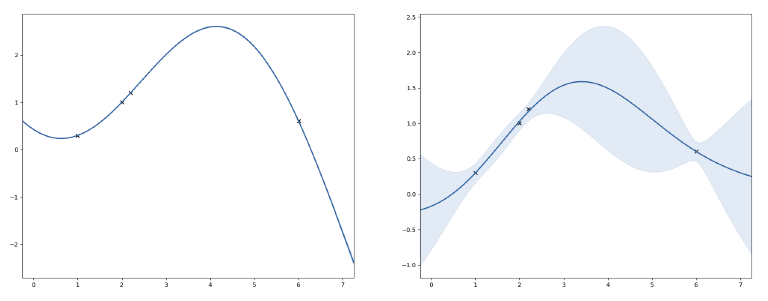
\includegraphics[height=0.4\textwidth]{images/GPh}}
\caption{Slika prikazuje Gausov proces s neoptimiziranimi parametri na levi in z optimiziranimi parametri na desni.}
\label{GP optimizacija hiperparametrov}
\end{figure}

\chapter{Odločilne funkcije}

\par V tem poglavju predstavimo uporabljene odločilne funkcije EI, PI in LCB in novejše funkcije kot so ES in KG ter jih umestimo na skalo med exploracijo in exploitacijo.
Za to poglavje predpostavimo, da želimo funkcije minimizirati, torej da je optimum funkcije v minimumu, v praksi to ni nujno zato pogosto preoblikujemo funkcijo v tako obliko, kjer to drži.

\section{Verjetnost izboljšave}

Verjetnost izboljšave ali PI je bila prva odločilna funkcije ustvarjena za Bayesovko optimizacijo. 
Predpostavimo, da je $f_{min}$ do zdaj najmanjša dosežena vrednost:

\begin{equation}
	f_{min} = min f
\end{equation}

Verjetnost izboljšave evaluira funkcijo $f$ v točki $x$, kjer je verjetnost največja. To je enakovredno naslednji funkciji $u$:

\begin{equation}
	u(x) = \left\{ \right.
\end{equation}

...

\chapter{Experimenti}

\section{Gradient Boosting}

Gradient Boosting je ML algoritem za regresijo in klasifikacijo problemov, ki ustvari napovedni model v obliki ansambla slabih napovednih modelov, tipično odločilnih dreves.


\newpage %dodaj po potrebi, da bo številka strani za Literaturo v Kazalu pravilna!
\ \\
\clearpage
\addcontentsline{toc}{chapter}{Literatura}

https://towardsdatascience.com/probability-concepts-explained-marginalisation-2296846344fc
https://machinelearningmastery.com/what-is-bayesian-optimization/
https://distill.pub/2020/bayesian-optimization/
http://krasserm.github.io/2018/03/19/gaussian-processes/
https://en.wikipedia.org/wiki/Multivariate normal distribution
https://peterroelants.github.io/posts/gaussian-process-tutorial/
https://en.wikipedia.org/wiki/Mat%C3%A9rn_covariance_function
https://towardsdatascience.com/radial-basis-function-rbf-kernel-the-go-to-kernel-acf0d22c798a
https://stats.stackexchange.com/questions/322523/what-is-the-rationale-of-the-mat%C3%A9rn-covariance-function

\end{document}

